%\documentclass{article}
\documentclass[paper=a4, fontsize=11pt, DIV=13]{scrartcl}

\usepackage{graphicx}
\usepackage{longtable}
\usepackage{amsmath}
\usepackage[T5]{fontenc}                           
\usepackage[utf8]{inputenc}
\usepackage{multirow}
\usepackage{listings}
\usepackage{color}
\usepackage{hyperref}

\usepackage{algorithm}
\usepackage{algorithmic}

\definecolor{codegreen}{rgb}{0,0.6,0}
\definecolor{codegray}{rgb}{0.5,0.5,0.5}
\definecolor{codepurple}{rgb}{0.58,0,0.82}
\definecolor{backcolour}{rgb}{0.95,0.95,0.92}
 
\lstdefinestyle{mystyle}{
    backgroundcolor=\color{backcolour},   
    commentstyle=\color{codegreen},
    keywordstyle=\color{magenta},
    numberstyle=\tiny\color{codegray},
    stringstyle=\color{codepurple},
    basicstyle=\footnotesize,
    breakatwhitespace=false,         
    breaklines=true,                 
    captionpos=b,                    
    keepspaces=true,                 
    numbers=left,                    
    numbersep=5pt,                  
    showspaces=false,                
    showstringspaces=false,
    showtabs=false,                  
    tabsize=2
}
\lstset{style=mystyle}

\begin{document}

\title{The Stony Brook Glad All Over Machine\\ Final Report}
\author{Trung Nguyen - 111752939
\\Anh Quang Do - 110922124
\\Nam Nguyen - 111171365}
\date{\today}
\maketitle
  
\section{Feature Engineering}

\subsection{MFCC Features} 
MFCCs features represent the envelope of the audio spectra and are the most widely used features for analyzing audio. The first 20 (the lower dimensions) of MFCC represents the envelope of spectra. And the discarded higher dimensions expresses the specral details. For different phonemes, envelopes are enough to represent the difference, so we can recognize phonemes through MFCC. In fact, the first 13 MFCC components is enough to solve a simple audio recognition task. In this problem, we used 20 first MFCC components.

In the progress report, we mentioned that each song in our dataset is represented by a 20x10000 matrix (called matrix M). Then, we take the mean of those 20 MFCCs to have a 20x1 feature vector for each song. However, by taking the mean, we have sacrificed much information from the audio files. 

Therefore, we solve this problems as follows: 

\begin{itemize}

\item We take a shorter time frame of 30 seconds where the highest notes are to analyze (from the 55th second to 85th second). We believe that by doing so, we are getting the most important part of the song to evaluate the singer, plus after taking the mean we won’t lose as much information. This also helps us processing the data much faster.

\item We do not only take the mean (20) but also take the covariance of 20 MFCCs (the upper triangular of covariance matrix) and get the number of features as: $20 + 20 \times 21/2 = 230$. Using these features, we obtain a better predicting result. 

\item Instead of the above approach, we also experimented another approach, which is instead of considering the whole 30 second time frame as one, we split it into 4 small time frame of 7.5 seconds each, and then take the mean of of each time frame, which ends up giving us $20 \times 4 = 80$ features.

The results of experimenting different feature sets over different problems are described in the later parts of this report.
\end{itemize}


\subsection{Using MFCCs to classify male and female voice}

We tried to investigate if the way we extract and use MFCCs as the main features is meaningful. In other words, we would like to make sure that our features are informative, which can be used for a simpler predicting task like distinguishing between female voice and male voice. We then solved a minor problem of binary classification (detecting male or female voice) by using logistic regression and support vector machine. The label male/female for each recording is the information we obtained from the singers from webscraper. The table below shows the accuracy of this task using the unprocessed data set with 2 above models. Because the number of recordings from female singers is larger, we randomly removed them until equal to the number of recordings from male singers (which will give us a probability of 0.5 if predict randomly)

As a matter of fact, using only 20 features (only means of MFCCs) we can classify male and female voice with the accuracy of 67\% (when using logistic regression) or 75\% (when using support vector machine). As expected, when using 230 features or 80 features model, we can differentiate between two kind of voice with the accuracy of more than 80\%. The accuracy of classification problem is summarized in the table below.

\begin{center}
 \begin{tabular}{|c | c c c|} 
 \hline
 Classifier & 20 Feautures  & 230 Features (Mean+Cov) & 80 Features (4 frames) \\ [0.5ex] 
 \hline\hline
 Logistic Regression & 0.6736 & 0.7973 & 0.8209 \\ 
 \hline
 Support Vector Machine & 0.7502 & 0.8108 & 0.8358 \\
 \hline
\end{tabular}
\end{center}
\begin{center}

\textit{Accuracy of classifying male/female using different features models}
\end{center}

It is worth to note that the best performance we have when using support vector machine is with parameter C = 300, which indicates a little bit "hard" and small margin, meaning the male and female voice are not tightly clustered. Though, the accuracy is enough to infer that our audio features are meaningful.

\section{Data Cleaning}

Our dataset contains 1921 instances. We did some preprocessing steps such as denoising and outlier removal, described in the next two sections. 

\subsection{Removing noise}
We have a dataset of nearly 2000 samples, however, a lot of them have little likes and views. Reasoning that, a sample with little likes and views may not be necessarily a “bad” cover, it may be due to the cover was not exposed to a lot of listeners, or it is a newly uploaded cover, we think that these data can be a noise to the model, since our score function will rate them as bad covers. After testing with several thresholds, we decided to remove samples with less than 10 views(and so, little likes), which is about 650 samples, to be our cutoff, so that we can reduce the noises in the data, but still managed to keep a reasonable number of samples for training.

We tested our model, and received a better result.

\subsection{Remove outliers}
In our dataset, there are two outliers as we can see from the proposal’ plot. These particular samples has exceptionally high score(high views and high likes). These outliers may affects our regression model performance a lot (especially the Linear Regression), since their likes and views are several times bigger than the rest. As a result, we decide to remove these samples out of the dataset, and we actually got a better training result, as we will show belows.

\section{Models}

\subsection{Considering the problem as Regression instead of Classification}
Our previous approach in this project is to form the problem as a classification one, which takes the input as a karaoke song, processes, then outputs the rating of this song from 1 to 5 stars. However, as the first try, we used a sub-dataset of just around 500 samples to speed up the training process, and our dataset is imbalanced (most of the songs are rated 2 stars) and the features are not enough to capture the song (only 20 means of MFCCs), the accuracy of our model is low (0.46).

As we use the full dataset of around 2000 samples, the accuracy of our multiple classification model is significantly improved (0.65). Seeing from the structure of the dataset. We then tested our model in a simpler problem, which is binary classification to discriminate between good and bad song and got the accuracy of 0.72.

Notwithstanding, we would like to form the problem in a different way, giving the absolute score to a song rather than put it to a bucket from 1 to 5. Thus, we tried different regression models, represented in the rest of this section, on the target, which is the scoring function that we defined as below.

\subsection{Scoring}
As mentioned in the proposal, we have several context features (which are based on social interaction such as numbers of likes, numbers of views to distinguish from content features, which are MFCCs) that we are inclined to take as the ground truth in our dataset to label the quality of the singing. 

In the progress report, we represented the number of likes and the number of views as a 2D-space and cluster the dataset into 5 regions corresponding to 5 ratings. Previously, our rating system reflects our subjective opinion that songs rated 1 star (lowest rating) would be songs with a little amount of likes but a large amount of views. That is to say, if x is a data point in a space spanned by the number of views and the number of likes, the score assigned to x is proportional to both ||x|| and arg(x) (arg(x) is large if x has more likes than views). 

However, after experiencing the singing by ourselves, we discovered that it is more appropriate if the score assigned to x is dependent on only ||x||. Expressed in a different way, score(x) would depend on (number of likes + number of view). Eventually, we decide to take this following scoring function for each singing piece x:
\begin{equation}
\text{score(x)} = \log(\text{\#views} + \text{\#likes} +1) \nonumber
\end{equation}

We observed that the number of views is more reliable than the number likes, which is a little noisy, but we do not use weighted sum since the numbers of like is mostly small (ranging from 0 to nearly 200) compared to the numbers of view (ranging from 0 to over 7000). After applying this scoring function, we got a score for each song in our dataset, ranging from 0 to 8.9. We did listen to several songs with different scores and conclude that the scoring is quite consistent, especially with songs with high score. The figure below shows the distribution of score for every songs in our training set.

\begin{center}
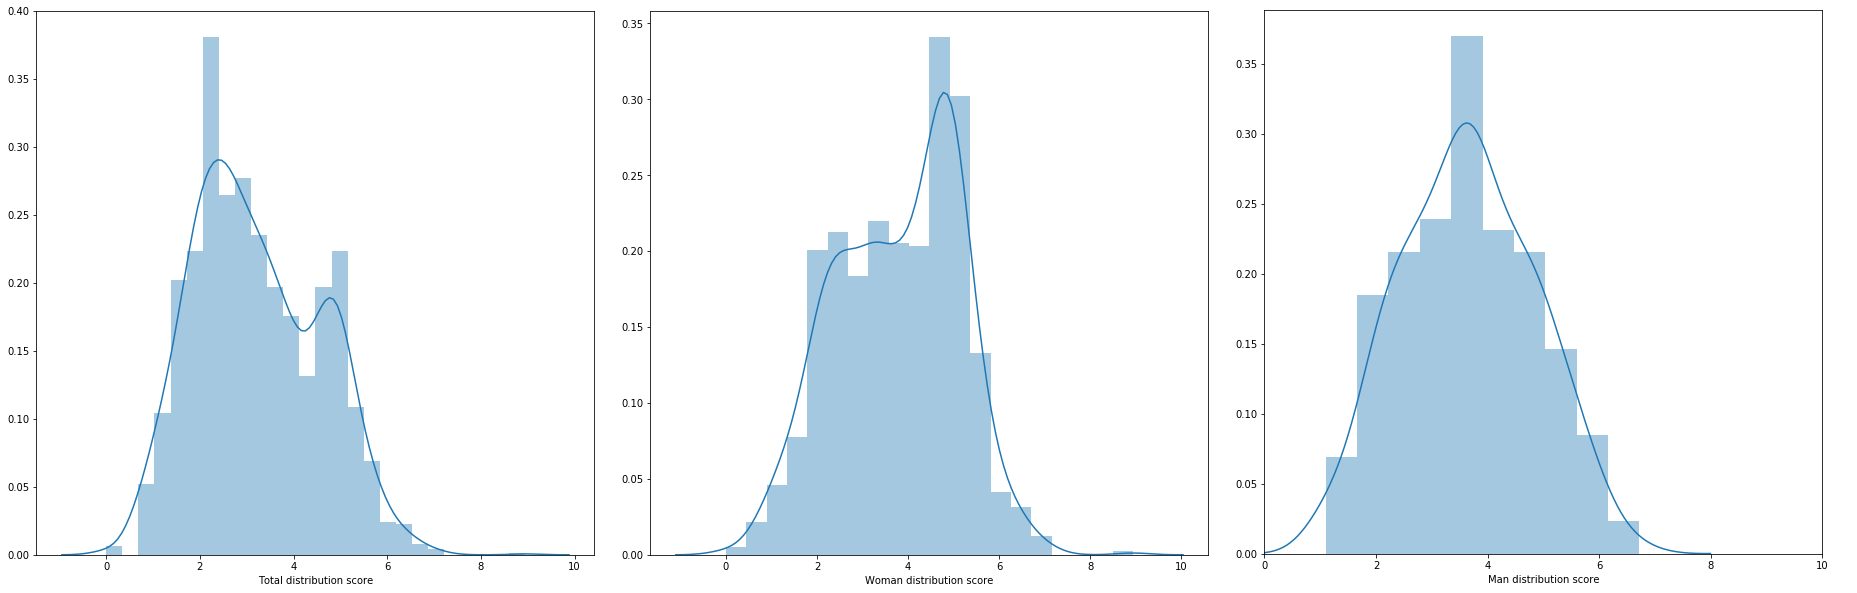
\includegraphics[scale=0.25]{img/1.png}\\
\textit{Distribution of scores from left to right: all - woman - man}\\
\end{center}

From the plot, we observe that the distribution is somewhat like a bimodal distribution. We reason for this phenomenon as there might be two distinct groups of users singing the song, one of which are popular users who have premium account of the recording website, the other of which are normal users who do not have premium account. Yet, when we plot the distribution of number of views over these two groups, there is still a bimodal distribution on premium account group. We then investigated if there is discrimination between male groups and female groups and actually found out that the two distributions based on gender are more “normal-like”. This would be justified since the karaoke song we took in our dataset is “My heart will go on”, which required a soprano, i.e. a female voice. Therefore, the group with large number of view might be female group and the other might be male group. Regardless, we first decide to use Gaussian Mixture Model in our regression model to capture the “two-mode” characteristic of the target (score).

\subsection{Gaussian Mixture Regression} 
We applied the GMM-GMR [1], which is a set of functions to train a Gaussian Mixture Model (GMM) and retrieve generalized data through Gaussian Mixture Regression (GMR). It allows to encode dataset in Gaussian Mixture Model (GMM) through Expectation-Maximization (EM) algorithms. By using this model, Gaussian Mixture Regression (GMR) can then be used to retrieve partial output data by specifying the desired inputs. It then acts as a generalization process that computes conditional probability with respect to partially observed data.
Our dataset is represented as $[X,y]$ where $X$ is audio features of songs (MFCCs) and y is songs’ score. The joint probability $p(X,y)$ is then encoded in GMM, and GMR is used to retrieve $p(y|X)$, namely the score given the audio features. Number of cluster we used to create an instance of GMM-GMR is 2, reflecting the two distinct groups. We got the MSE of 1.01 when using 230 features.

We then tried to fit another non-linear regression model which is Decision Tree.

\subsection{Decision Tree Regression}
We model our problem as a set of decision rules where the score of a song (quality) is based on some threshold of MFCCs’ values. A decision tree splits the input features (MFCCs) in several regions and assigns a prediction value (score) to each region. The selection of the regions and the predicted value within a region are chosen in order to produce the prediction which best fits the data (using mean square error).

We tried different value of the parameter maxDepth and a two-level tree (maxDepth = 2) gives us the best results, whose mean square error is 0.81 (when using 230 features)

That Decision Tree outperforms Gaussian Mixture Model and that Decision Tree is easily overfitted on our dataset (trees with maxDepth greater than 2 delivered bigger error) indicates that our dataset is not too far from linearity. Thus, we gave Linear Regression a try.

\subsection{Linear Regression (Baseline Model)}
The reason why we do not use Linear Regression from the start is because the distribution of target value (score) is not normal and will affect the performance of linear regression. However, we then learned that the only distribution matters in this case is the distribution of residuals (errors), not of the data itself. Therefore, we fit a linear regression and plot the residual errors to see if it is a normal distribution. We got a mean square error of 1.04 from scores ranging from 0-7.1 and the residual plot in the figure below shows that the errors are randomly scattered around line zero, which indicates that using linear regression is quite reasonable. 

\begin{center}
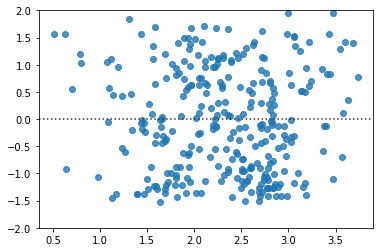
\includegraphics[scale=0.9]{img/2.png}\\
\textit{Residual plot of MSE}\\
\end{center}

As stated by No Free Lunch Theorem, we could not expect models which are more complex than linear model will perform better. Inversely, the principle of Occam’s razor shows that the simplest model among all would be the best; linear regression is simple but still a very effective predictive model. In fact, in our case, the performance of linear regression is not far behind the other two models above. Yet, we still can have a simpler and more effective model by regularizing it.

\subsection{L1 Regularization}
We used the L1-regularizer (LASSO) on linear regression because it provides a sparse solution, which means reducing the number of features. Although the distribution of the error as a function of the number of features and sample size is unknown in general, there is an heuristic depicting that as feature correlation increases, the optimal feature size becomes proportional to $\sqrt{N}$ (where N is sample size) for highly correlated features [2]. Our dataset contains approximately 2000 samples (N) and 230 features, which larger than 45 ($\sqrt{N}$) so we might suffer the curse of dimensionality if not using the L1-regularizer. The other reason for using L1-norm is that some model using it has a sample complexity that grows logarithmically with the number of features [3].

After fitting the LASSO model, we have a better performance, whose mean square error is 0.76. We also reduce 96 features from our dataset.

\subsection{AdaBoost and Gradient Boosting}

We then try to boosting our model using AdaBoost and Gradient Boosting as in the next sections.

As mentioned in previous sections, the complex models might overfit our data. However, our linear model could also suffer the underfit problem; in other word, linear model could also be a weak learner (as decision stumps). The appropriate way to enrich our model (the hypothesis space) is to slightly increase our model complexity to avoid both underfitting and overfitting problem. This is could be done with AdaBoost meta-algorithm, which allows us to construct non-linear classifiers one piece at the time. The basic idea of boosting is to use a weak learning algorithm that provides "rough rules-of-thumb" to construct a very accurate predictor. The mean square error of using AdaBoost and Gradient Boosting are 0.69 and 0.65 respectively. We could see that they outperform the Lasso Regression; Gradient Boosting performs the best.

\subsection{Iterative Algorithm (on going approach)}
As a matter of fact, the problem we faced with the dataset when taking views and likes as ground truth is that it is noisy. We experienced that while the singing pieces with large number of view and like are good, it is hard to distinguish between pieces with small number of view and like, which are the majority in our dataset. Therefore, we proposed an algorithm to iteratively fit the model and update the score of our dataset until some convergence condition is satisfied.  Normally, the algorithm will be converged when there is no more change in the score; however, this could lead to overfitting problem. Thus, we will define some threshold of the difference between score and target for the iteration to be stopped.

We define a scoring function on number of like and view, parameterized by weight: 
$g(w_1, w_2) = log(w_1*like + w_2*view)$ and a fitting model f (for example, a linear regression $f(w,b; g)$), then the algorithm is described as follow:

\begin{algorithm}
\caption{Iterative Algorithm}
\begin{algorithmic} 

\STATE Initialize $w_1 = w_2 =1$
\STATE Threshold = 0.1 
\WHILE{$(sum|y - g(w_1, w_2)| \leq threshold)$}
\STATE 1. Fit $f(w,b; X,y)$
\STATE 2. $y \gets X*w + b$
\STATE 3. $(w_1,w_2) \gets g^{-1}(y)$
\STATE 4. $y \gets g(w_1, w_2)$
\ENDWHILE

\STATE Output $g(w_1, w_2)$ and $f(w,b)$

\end{algorithmic}
\end{algorithm}

\section{Evaluation}
The results (mean square error) of all our models are summarized in the table below. We could see that when using 230 feature (i.e. consider the covariance of 20 MFCCs), the performance of all models are much better. Also, the baseline model (linear regression) has the lowest and the Gradient Boosting (GB) has the highest performance. However, we could see that Gaussian Mixture Regression (GMR) and Decision Tree Regression (DTR) do not work well with 80 features (i.e. no covariance of MFCCs). Their performance is even worse than baseline model.

\begin{center}
 \begin{tabular}{|c| c c c c c c c|} 
 \hline
 Regressor 
& Linear
& GMR
& DTR
& Lasso
& Ada
& GB
  \\ [0.5ex] 
 \hline\hline
 230 Features 
& 1.04
& 1.01
& 0.81
& 0.76
& 0.69
& 0.65
 \\ 
 \hline
 80 Features 

& 1.17
& 1.67
& 1.41
& 1.10
& 1.14
& 1.05
 \\
 \hline
\end{tabular}
\end{center}

\section{Conclusion and Future Works}

Our approach in this Music Information Retrieval (MIR) project is to combine the content features, i.e. audio features (MFCCs, etc.) and context features, e.g. number of like and view, etc. to build a model which can detect the quality of a record. While it is not hard to detect some basic quality like gender (male vs. female voice), it is not easy to detect a good singing voice. In this report, we presented some supervised methods and results to generate score to a singing piece. 

We also built a prototype system in which people can record their singing and then retrieve the score after the singing piece is analyzed inside the system. Due to the fact that the context features, especially the ones which can indicate good singing, are noisy, we would consider the semi-supervised approach in the future.

Furthermore, We face a technical problem in which we would like to, but not really successfully extract the vocal from the background music. We tried to do so with some available script and tools, e.g. Audacity, but the results are only singing pieces with lower volume. However, we would like to explore another approach in the future, which is manifold alignment [4] [5]. To avoid splitting vocal from background music, our basic idea is to align two or more singing pieces of the same song using traditional method like Dynamic Time Warping [6] or based on Manifold Learning like Manifold Warping [7]. Next, if we can project these singing pieces in a common manifold, we could then rank them appropriately [8].

Finally, since our problem is heavily dependent on the sensation of the listeners, we would like to have a survey in the next few days when we can gather enough people, ask them to listen to songs and give scores to them, then compare the results with our predicted scores.

\begin{thebibliography}{99}

\bibitem[1] hhttps://github.com/BatyaGG/Gaussian-Mixture-Models
\bibitem[2] HHua, Jianping, et al. "Optimal number of features as a function of sample size for various classification rules." Bioinformatics 21.8 (2004): 1509-1515.
\bibitem[3] NNg, Andrew Y. "Feature selection, L 1 vs. L 2 regularization, and rotational invariance." Proceedings of the twenty-first international conference on Machine learning. ACM, 2004.
\bibitem[4] WWang, Chang, and Sridhar Mahadevan. "Manifold alignment using procrustes analysis." Proceedings of the 25th international conference on Machine learning. ACM, 2008.
\bibitem[5] PPlummer, Andrew R., et al. "Learning speaker normalization using semisupervised manifold alignment." Eleventh Annual Conference of the International Speech Communication Association. 2010.
\bibitem[6] BBerndt, Donald J., and James Clifford. "Using dynamic time warping to find patterns in time series." KDD workshop. Vol. 10. No. 16. 1994.
\bibitem[7] VVu, Hoa Trong, Clifton Carey, and Sridhar Mahadevan. "Manifold Warping: Manifold Alignment over Time." AAAI. Vol. 1. No. 4. 2012.
\bibitem[8] QQin, Jing, Xinyue Liu, and Hongfei Lin. "Audio Retrieval Based on Manifold Ranking." Parallel Architectures, Algorithms and Programming (PAAP), 2014 Sixth International Symposium on. IEEE, 2014.

\end{thebibliography}

\end{document}